\section{Test Case}
\label{sec:testCase}

\subsection{Plant Description}
For our analysis we have chosen a 3-unit plant as shown in Fig.~\ref{fig:layout}. The chosen layout 
is not representative of any existing plant but it is simply fictitious.
From a topographical perspective, a large body of water is located in proximity of the NPP and it is 
employed as ultimate heat-sink for the plant.

\begin{figure}
    \centering
    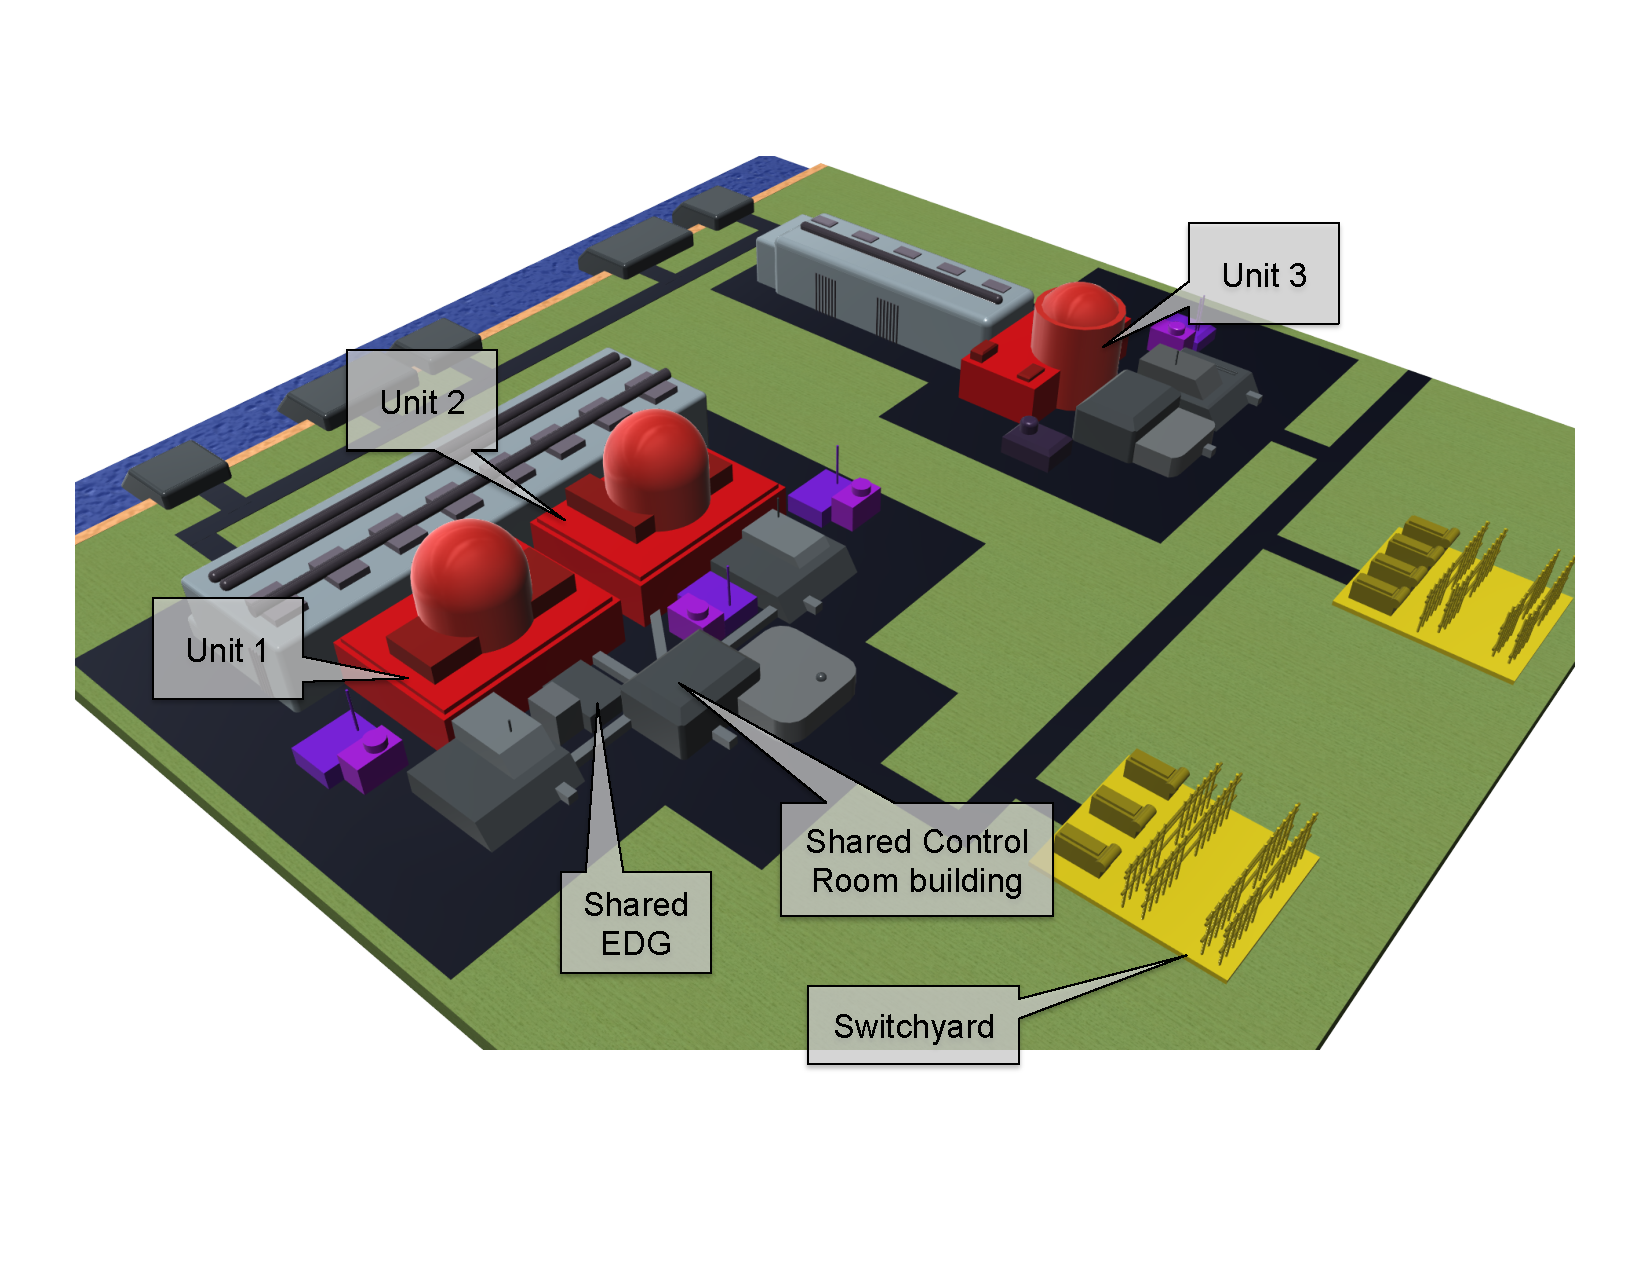
\includegraphics[scale=0.5]{layout.pdf}
    \caption{Overview of the multi-unit plant}
    \label{fig:layout}
\end{figure}

All three units are composed by PWR systems (see Fig.~\ref{fig:PWRscheme}); the design of the PWR systems 
are identical for all the three units and it 
can be considered generic, i.e., it is not specific to an existing plant. 

\begin{figure}
    \centering
    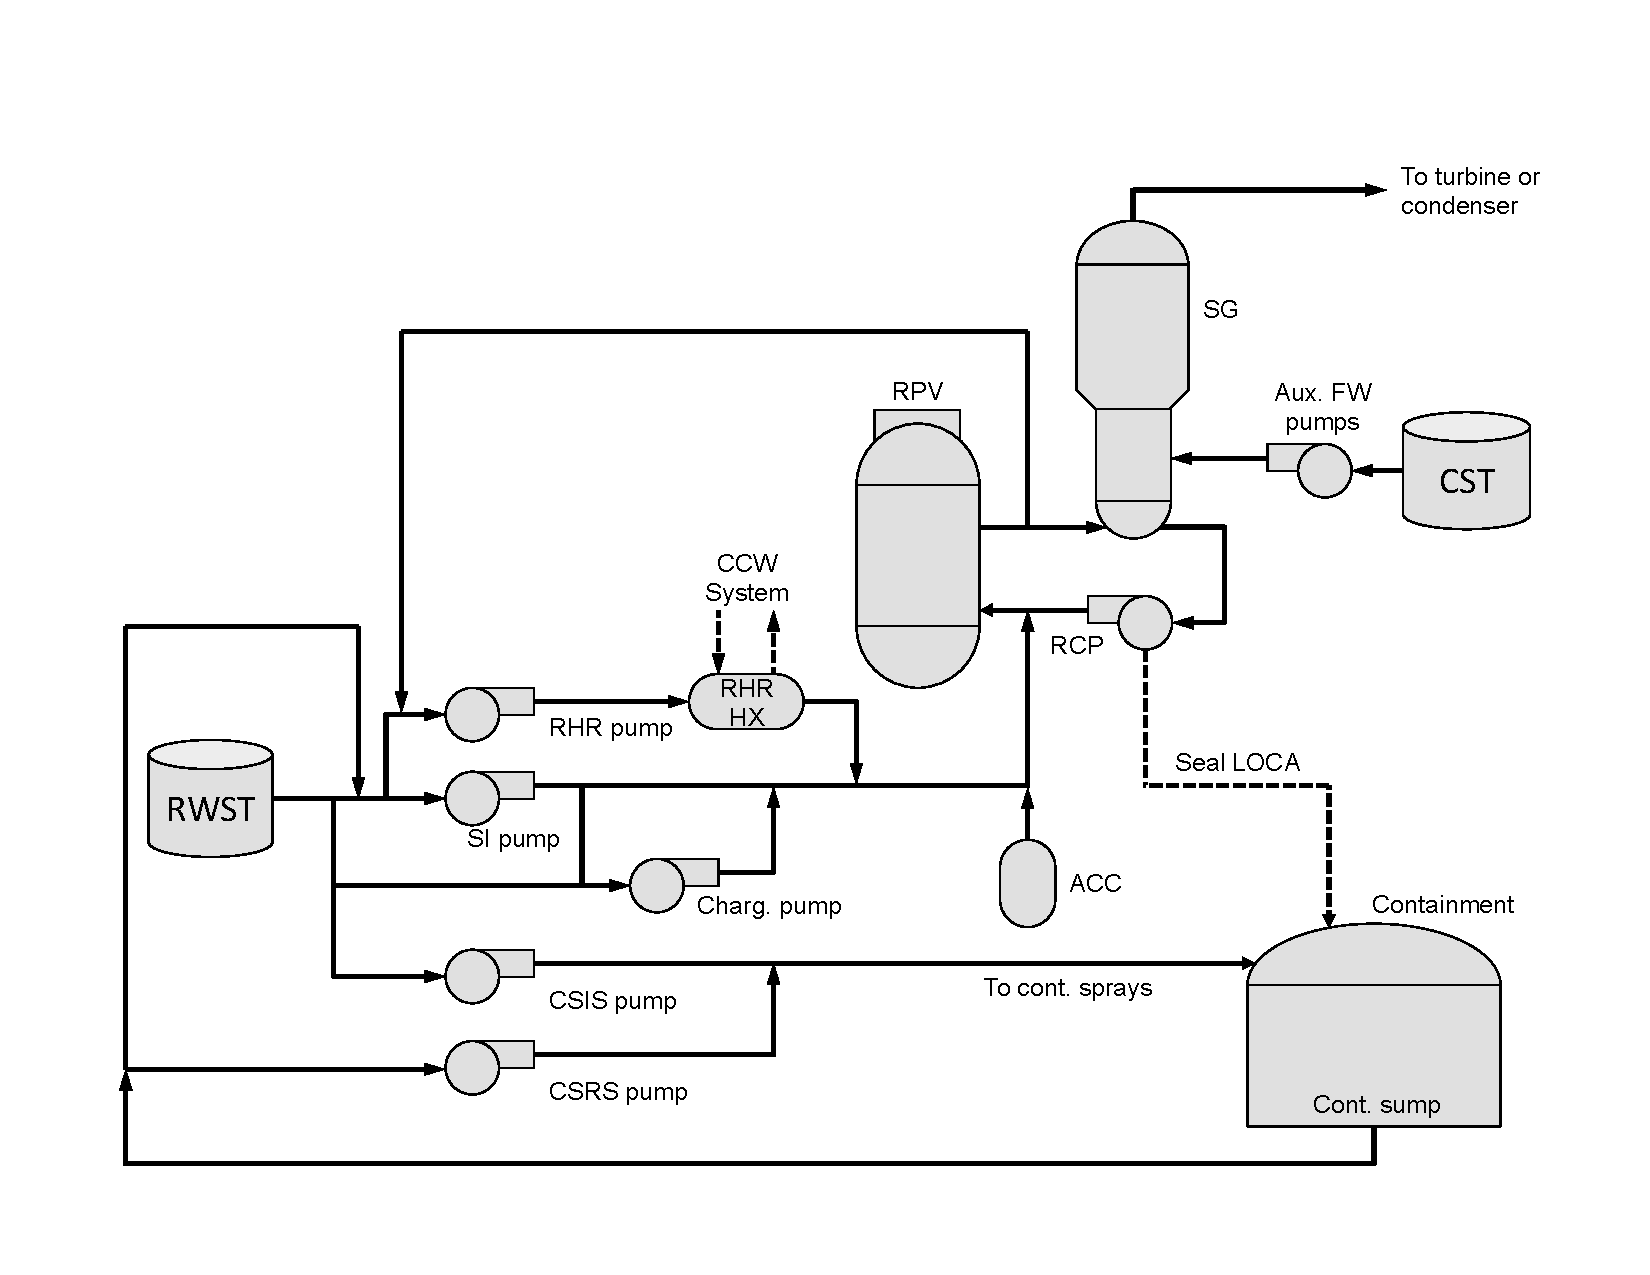
\includegraphics[scale=0.5]{PWRscheme.pdf}
    \caption{Generic scheme of a PWR system}
    \label{fig:PWRscheme}
\end{figure}

\begin{figure}
    \centering
    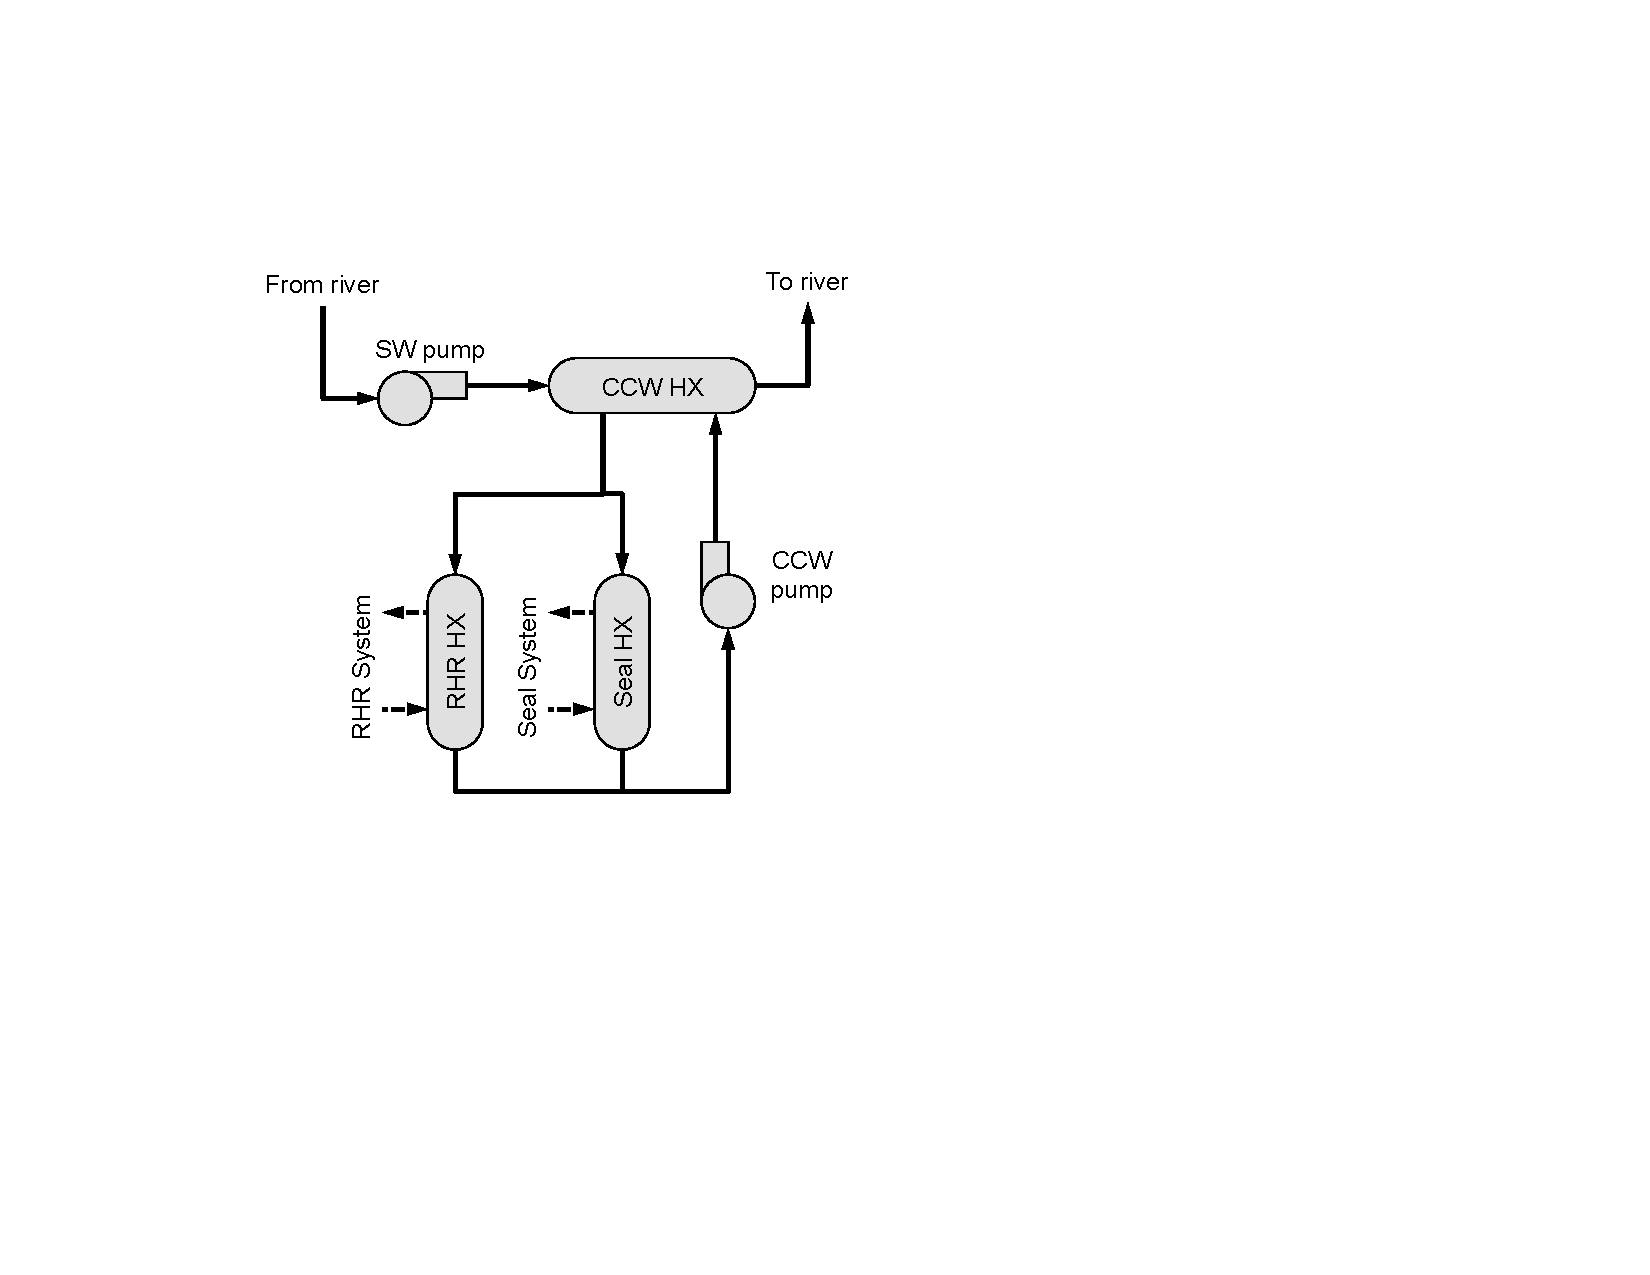
\includegraphics[scale=0.5]{CCW-SW.pdf}
    \caption{Generic scheme of a the CCW and SW systems}
    \label{fig:CCW-SWscheme}
\end{figure}

For each PWR, the systems considered in the analysis are the following:
\begin{itemize}
  \item High Pressure Injection System (HPIS)
  \item Low Pressure Injection System (LPIS)
  \item Residual Heat Removal (RHR) system
  \item Accumulators (ACCs)
  \item Auxiliary Feed-water (AFW) system 
  \item Charging pumps
\end{itemize}

Special attention has been given to the design of the electrical and hydraulic systems:
\begin{itemize}
  \item The plant electrical system is shown in Fig.~\ref{fig:electricalScheme}. Two electrical switch-yards can 
        provide electrical power to all units. All units have a set of Emergency Diesel Generators (EDGs) 
        and, in addition, a swing EDG (i.e., EDGS) can be employed to provide an alternate AC power to either
        Unit 1 or Unit 2. Note also that the 6.6 KV emergency buses of Unit 1 and Unit 2 can be cross-tied.
  \item The auxiliary feed-water (AFW) system of Unit 1 and Unit 3 can be cross-tied. Thus cooling to the 
        secondary side can be provided from one unit to the other one.
  \item The Condensate Storage Tanks (CSTs) of Units 2 and Unit 3 can be cross-tied. Thus the water source 
        for the secondary side of either unit can be used as water source for the other one. 
        \item Plant recovery crew is a shared resource within the plant. As part of the accident scenario, 
        the recovery crew can perform AC power and safety injection using mobile equipment located within each unit.
\end{itemize}

\begin{figure}
    \centering
    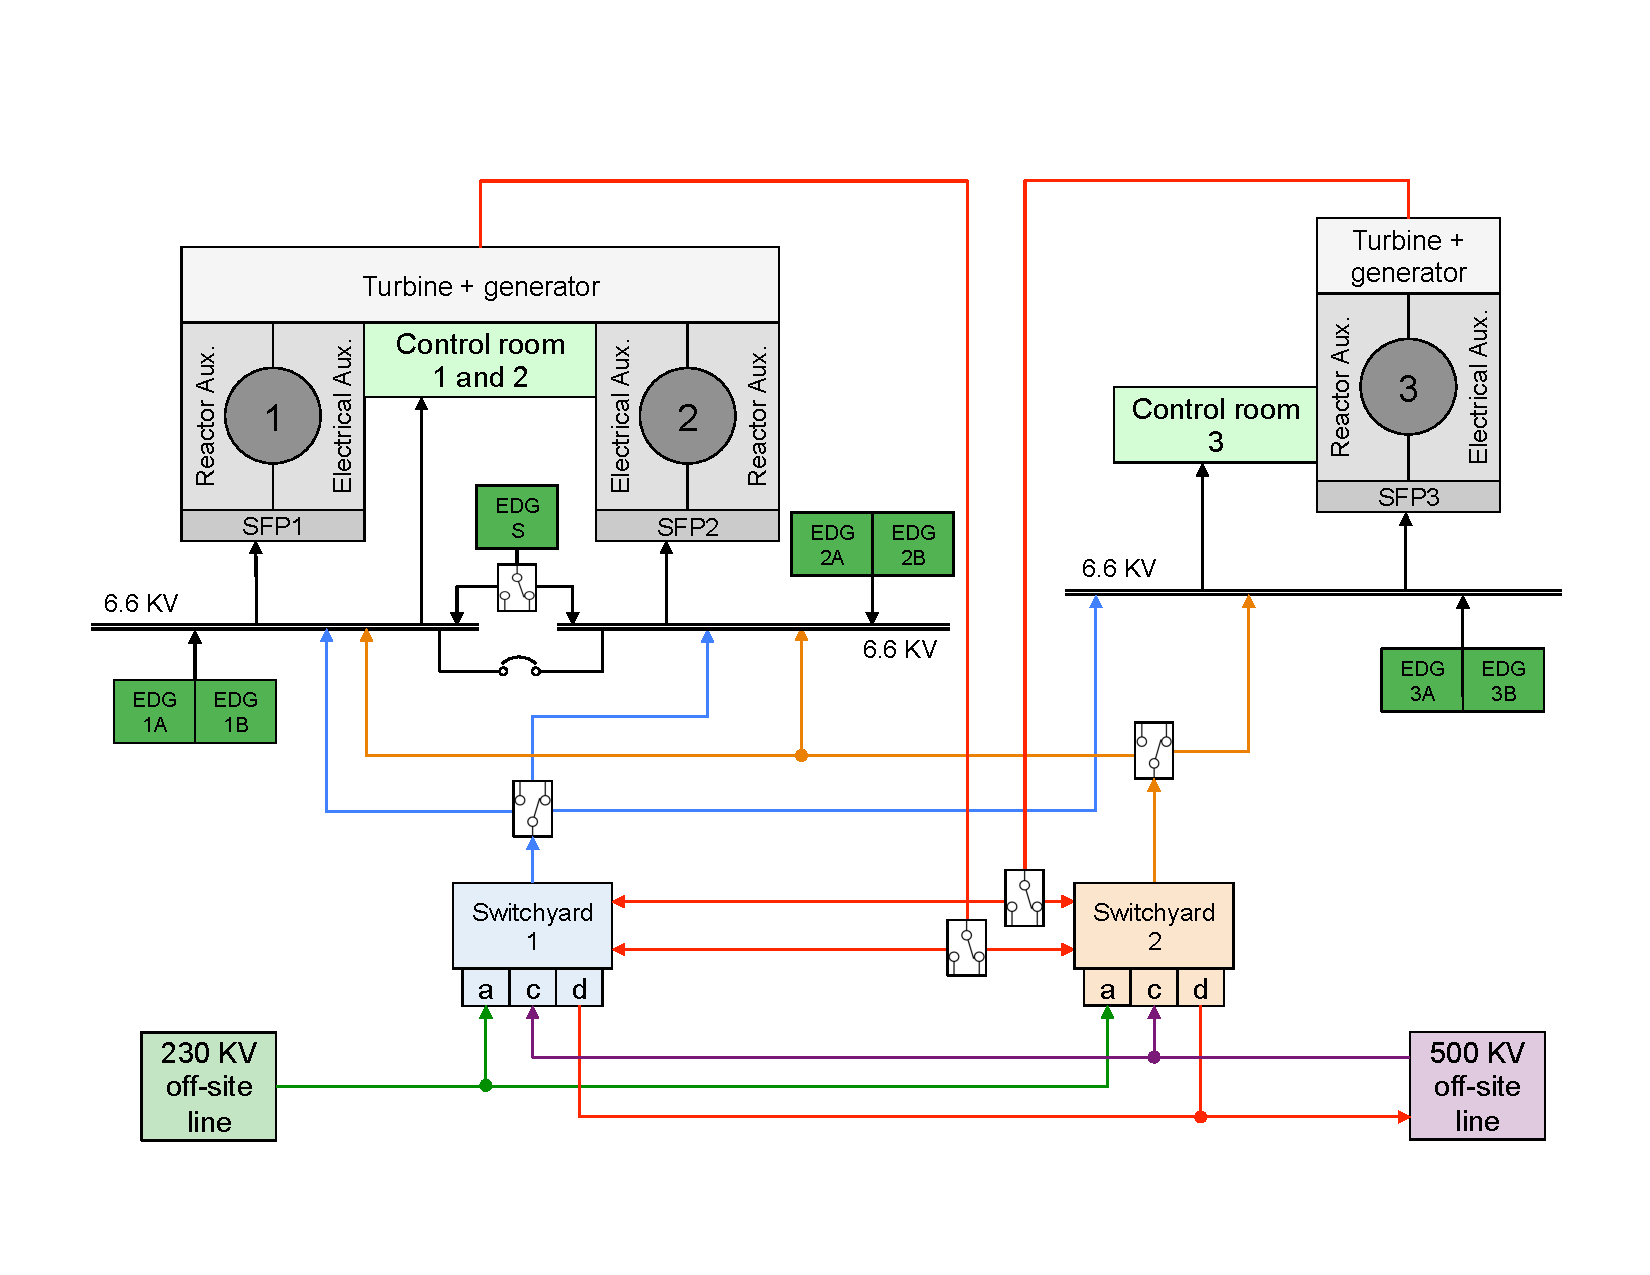
\includegraphics[scale=0.5]{electricalScheme.pdf}
    \caption{Overview of the plant electrical scheme}
    \label{fig:electricalScheme}
\end{figure}


\subsection{Initiating Event}

The considered accident scenario is a seismic event which causes the following events:
\begin{itemize}
  \item Both switch-yards are disabled
  \item All EDGs are disabled except EDGS which is initially aligned to Unit 2
  \item CST of Unit 2 has lost 80\% of its capacity 
  \item CST of Unit 3 is completely lost
  \item The seismic event might also rupture the SFPs. Thus a leak might be present during the accident scenario
\end{itemize}

The proposed accident scenario resembles a Station Black Out (SBO) event at the plant level except for the 
fact that the EDGS is the only source of AC power available and it can be directed toward either Unit 1 or Unit 2.

Prior the seismic event, the three units initial conditions are summarized in Table~\ref{tab:unitsStatus}:

\begin{table}
  \begin{tabular}{ | l | p{10cm} | }
    \hline      
      Unit 1 &  The PWR of Unit 1 (i.e., PWR1) is at full power (100\% power level) and it own SFP \\ \hline
      Unit 2 &  The PWR of Unit 2 (i.e., PWR2) is in mid-loop operation (i.e., shut-down mode) and it own SFP. 
                The mid-loop status is characterized by a primary coolant system drained to the 
                hot leg centerline and the existence of openings which a further reduction of 
                the mass inventory poses a serious risk, due to boil off and possible entrainment 
                or spill over of liquid\\ \hline
      Unit 3 &  The PWR of Unit 3 (i.e., PWR3) is at full power (108\%) that restarted a few weeks 
                earlier and its own SFP with a higher heat load since it contains used fuel recently 
                moved from the reactor. \\
    \hline  
  \end{tabular}
  \caption{Initial status of the three unit prior the accident scenario}
  \label{tab:unitsStatus}
\end{table}


